\documentclass[11pt]{article}

\usepackage{mathtools}
\usepackage{float}
\usepackage{amssymb}
\usepackage{amsmath}
\usepackage{amsthm}
\usepackage{hyperref}
\usepackage{microtype}
\usepackage{graphicx}
\usepackage{blkarray}
\usepackage{pgfplots}
\pgfplotsset{compat=1.15}
\usepackage{mathrsfs}
\usetikzlibrary{arrows}
\graphicspath{ {./img/} }
\pagestyle{empty}

\setlength{\parindent}{0cm}
\let\emptyset\varnothing

\title{\textbf{CSCI/MATH 2113 Discrete Structures} \\ Appendix 3 Countable and Uncountable Sets}
\author{Alyssa Motas}

\begin{document}

    \maketitle

    \pagebreak

    \tableofcontents

    \pagebreak

    \section{Cardinality}

    \emph{Counting:} Typical questions include:
    \begin{itemize}
        \item What is \(|A|\)?
        \item Is it the case that \(|A| < |B|?\)
        \item Is it the case that \(|A| = |B|?\)
    \end{itemize}

    For finite sets, we have 
    \begin{itemize}
        \item Count \(|A|\), say \(|A| = n\). 
        \item Count \(|B|\), say \(|B| = m\).
        \item Compare $n$ and $m$.
    \end{itemize}

    What about for infinite sets? How do \(|\mathbb{N}|\) and \(|\mathbb{Z}|\) compare? What about \(|\mathbb{N}|\) and \(|\mathbb{R}|\)?

    \subsection{Definition of bijection}

    For any nonempty sets $A,B$ the function \(f:A \rightarrow B\) is called a \emph{one-to-one correspondence} if $f$ is both one-to-one and onto.

    \subsection{Definition of same cardinality}

    If $A,B$ are two nonempty sets, we say that $A$ \emph{has the same size, or cardinality}, as $B$ and we write $A \sim B$, if there exists a one-to-one correspondence \(f:A \rightarrow B\).

    \vspace{1em}

    \emph{Example:} \(|\mathbb{N}| = |2 \mathbb{N}| = \{n \in \mathbb{N} \mid \text{$n$ is even}\}\). To see this, consider the function \(f: \mathbb{N} \rightarrow 2 \mathbb{N}\). We have 
    \begin{itemize}
        \item \(f(n) = f(m) \Rightarrow 2n = 2m \Rightarrow n = m\), so $f$ is injective.
        \item \(x \in 2 \mathbb{N} \Rightarrow x = 2y\) for \(y \in \mathbb{N} \Rightarrow f(y) = x \Rightarrow f\) is surjective.
    \end{itemize}
    Another example is \(|\mathbb{N}| = |3 \mathbb{N}|\) since \(g: \mathbb{N} \rightarrow 3 \mathbb{N}\).

    \subsection{Properties of sets}

    Let \(A,B,C\) be sets. Then:
    \begin{itemize}
        \item \(|A| = |A|\)
        \item \(|A| = |B| \Rightarrow |B| = |A|\)
        \item \(|A| = |B|\) and \(|B| = |C| \Rightarrow |A| = |C|\).
    \end{itemize}

    \begin{proof}
        \begin{itemize}
            \item \(1_{A}: A \rightarrow A\) is bijective.
            \item If \(|A| = |B|\), then \(\exists f:A \rightarrow B\) bijection \(\Rightarrow\) $f$ is invertible \(\Rightarrow f^{-1}:B \rightarrow A\) is invertible \(\Rightarrow \exists g: B \rightarrow A\) bijective \(\Rightarrow |B| = |A|\).
            \item \(|A| = |B|\) and \(|B| = |C|\)
            \begin{align*}
                &\Rightarrow \exists f:A \rightarrow B, \exists g:B \rightarrow C \text{ both bijective} \\
                &\Rightarrow g \circ f:A \rightarrow C \text{ is bijective} \\
                &\Rightarrow \exists h:A \rightarrow C \text{ bijective} \\
                &\Rightarrow |A| = |C|.
            \end{align*} 
        \end{itemize}
    \end{proof}

    \subsection{Finite and infinite sets}

    Any set $A$ is called a \emph{finite} set if \(A = \emptyset\) or if \(|A| = |\{1,2,3,\dots,n\}|\) for some \(n \in \mathbb{Z}^+\). When \(A = \emptyset\) we say that $A$ has no elements and write \(|A| = 0\). In the latter case, $A$ is said to have $n$ elements and we write \(|A| = n\). When a set $A$ is \emph{not} finite, then it is called \emph{infinite}.

    \vspace{1em}

    \emph{Question:} Is it the case that \(A,B\) infinite \(\Rightarrow |A| = |B|?\) Nope.

    \subsection{Countable}

    A set $A$ is called \emph{countable} (or \emph{denumberable}) if (1) $A$ is finite or (2) \(|A| = |\mathbb{Z}^+|.\)

    \vspace{1em}

    \emph{Examples:}
    \begin{itemize}
        \item \(2\mathbb{N}\) and \(3\mathbb{N}\) are countable.
        \item \(\mathbb{Z}\) is countable. Define \(f: \mathbb{N} \rightarrow \mathbb{Z}\) by \[f(x) = \begin{cases}
            \dfrac{x}{2} & \text{if $x$ is even} \\
            - \left(\dfrac{(x+1)}{2}\right) & \text{if $x$ is odd.}
        \end{cases}\] We show that $f$ is injective: Suppose \(f(x) = f(y)\). 
        \begin{itemize}
            \item If $x$ and $y$ are even, then \[f(x) = \frac{x}{2} = \frac{y}{2} = f(y)\] so \(x = y\).
            \item If $x$ and $y$ are odd, then \[f(x) = - \frac{x+1}{2} = - \frac{y+1}{2} = f(y)\] so \(x = y\).
            \item If $x$ is odd and $y$ is even, then \[f(x) = - \frac{x+1}{2} = \frac{y}{2} = f(y) \Rightarrow y = -x - 1\] but \(-x - 1 < 0\) and \(y \geq 0\) so this is a contradiction.
        \end{itemize}
        Thus, $f$ is an injection. Show that $f$ is a surjection: for all \(y \in \mathbb{Z}\) we have
        \begin{itemize}
            \item If \(y=0\), then \(f(1) = 0\)
            \item If \(y > 0\), then \(2y \in \mathbb{Z}^+\) and \(f(2y) = \frac{2y}{2} = y\)
            \item If \(y<0\), then \(-2y + 1 \in \mathbb{Z}^+\) and \(f(-2y + 1) = -[(-2y+1) - 1]/2 = -(-2y)/2 = y.\)
        \end{itemize}
        Therefore, $f$ is a surjection and \(|\mathbb{N}| = |\mathbb{Z}|\). 
    \end{itemize}

    \subsection{Finite and infinite sequence}

    For \(n \in \mathbb{Z}^+\), a \emph{finite sequence of n terms} is a function $f$ whose domain is \(\{1,2,3,\dots, n\}\). Such a sequence is usually written as an \emph{ordered} set \(\{x_1, x_2, x_3, \dots, x_n\}\), where \(x_i = f(i)\) for all \(1 \leq i \leq n\). 

    An \emph{infinite sequence} is a function $g$ having \(\mathbb{Z}^+\) as ots dp,aom. This type of sequence is generally denoted by the \emph{ordered} set \(\{x_i\}_{i \in \mathbb{Z}^+}\) or \(\{x_1, x_2, x_3, \dots\}\), where \(x_i = g(i)\) for all \(i \in \mathbb{Z}^+\).

    \subsection{Sequence of distinct elements}

    If $A$ is a nonempty countable set, then $A$ can be written as a sequence of distinct elements.

    \subsection{Subset of an infinite countable set is countable}

    If $S$ is a countable set and \(A \subseteq S\), then $A$ is countable. 

    \begin{proof}
        When $S$ is finite, this is clear. When $S$ is infinite, then
        \begin{itemize}
            \item if $A$ is finite, there is nothing to show.
            \item if $A$ is infinite then we define a bijection from \(\mathbb{N}\) to $A$. 
        \end{itemize}
        Let \(f: \mathbb{N} \rightarrow S\) be a bijection (which exists by assumption). Define \(\overline{f}:\mathbb{N} \rightarrow A\) \[\overline{f}(0) = f(n_0) \text{ where } n_0 = \text{min} \{n \in \mathbb{N} \mid f(n) \in A\}\] \[\overline{f}(1) = f(n_1) \text{ where } n_1 = \text{min}\{n \in \mathbb{N} \setminus \{n_0\} \mid f(n) \in A\}.\] In general, \[\overline{f}(k) = f(n_k) \text{ where } n_k = \text{min} \{n \in \mathbb{N} \setminus \{n_{k-1}\} \mid f(n) \in A\}.\]
    \end{proof}

    \emph{Corollary:} If \(\exists f: A \rightarrow \mathbb{N}\) injective then $A$ is countable.

    \begin{proof}
        Then \(f[A] \subseteq \mathbb{N}\) and \(|A| = |f[A]|\). So, $A$ is countable.
    \end{proof}

    \subsection{Cantor's diagonal argument}

    The set \((0,1] = \{x \mid x \in \mathbb{R} \text{ and } 0 < x \leq 1\}\) is not a countable set. 
    \begin{proof}
        If \((0,1]\) were countable, then we could write this set as a sequence of distinct terms: \((0,1] = \{r_1, r_2, r_3, \dots\}\). To avoid two representations we agree to write real numbers in \((0,1]\) such as 0.5 as \(0.499\dots\) So, no element in \((0,1]\) is represented by a decimal expansion that terminates. We have 
        \begin{align*}
            r_1 &= 0.a_{11} a_{12} a_{13} a_{14} \dots \\
            r_2 &= 0.a_{21} a_{22} a_{23} a_{24} \dots \\
            r_3 &= 0.a_{31} a_{32} a_{33} a_{34} \dots \\
            \vdots & \\
            r_n &=  0.a_{n1} a_{n2} a_{n3} a_{n4} \dots \\
            \vdots &
        \end{align*}
        where \(a_{ij} \in \{0,1,2,3,\dots, 8, 9\}\) for all \(i,j \in \mathbb{Z}^+\). 

        Consider the real number \(r = 0.b_1 b_2 b_3, \dots\), where for each \(k \in \mathbb{Z}^+\),
        \begin{equation*}
            b_k = \begin{cases}
                3, & \text{if } a_{kk} \neq 3 \\
                7, & \text{if } a_{kk} = 3.
            \end{cases}
        \end{equation*}
        Then \(r \in (0,1)\), but for \emph{every} \(k \in \mathbb{Z}^+\), we have \(r \neq r_k\). So, \(r \notin \{r_1, r_2, r_3, \dots\}\). This contradicts our assumption that \((0,1] = \{r_1, r_2, r_3, \dots\}\).
    \end{proof}

    \emph{Corollary:} \(|(0,1]| \neq |\mathbb{N}|\). In fact, \(|(0,1]| > |\mathbb{N}|\). When a set is not countable, it is termed \emph{uncountable}. So, \((0,1]\) is uncountable.

    \vspace{1em}

    \emph{Corollary:} The set \(\mathbb{R}\) (of all real numbers) is an uncountable set.
    \begin{proof}
        If \(\mathbb{R}\) were countable, then the subset \((0,1]\) would be countable.
    \end{proof}
    
    \emph{Remark:} If \(X \subseteq S\), then
    \begin{itemize}
        \item if $S$ is countable, then $X$ is countable;
        \item if $X$ is uncountable, then $S$ is uncountable.
    \end{itemize}

    \emph{Examples:}
    \begin{itemize}
        \item \(\mathbb{N} \subseteq \mathbb{Q}\) and \(\mathbb{Q} \subseteq \mathbb{R}\).
        \item \(\mathbb{R} \subseteq \mathbb{C}\) so \(\mathbb{C}\) is uncountable.
        \item \(\mathbb{R} \subseteq \mathbb{R} \cup \{i\}\) so \(\mathbb{R} \cup \{i\}\) is uncountable. 
    \end{itemize}

    \pagebreak

    \subsubsection{Example}

    Consider the points in the Cartesian plane on the unit circle \(x^2 + (y-1)^2 = 1.\) How large is this set \(S = \{(x,y) \mid x,y \in \mathbb{R} \text{ and } x^2 + (y-1)^2 = 1\}\)? That is, is $S$ countable or uncountable?
        
    We have a unit circle centered at \(C(0,1)\). This circle is tangent to the real number line (or $x$-axis) at the point where \(x = 0\). The point $P$, on the circumference, has coordinates \((0,2)\). 

    \begin{figure}[H]
        \centering
        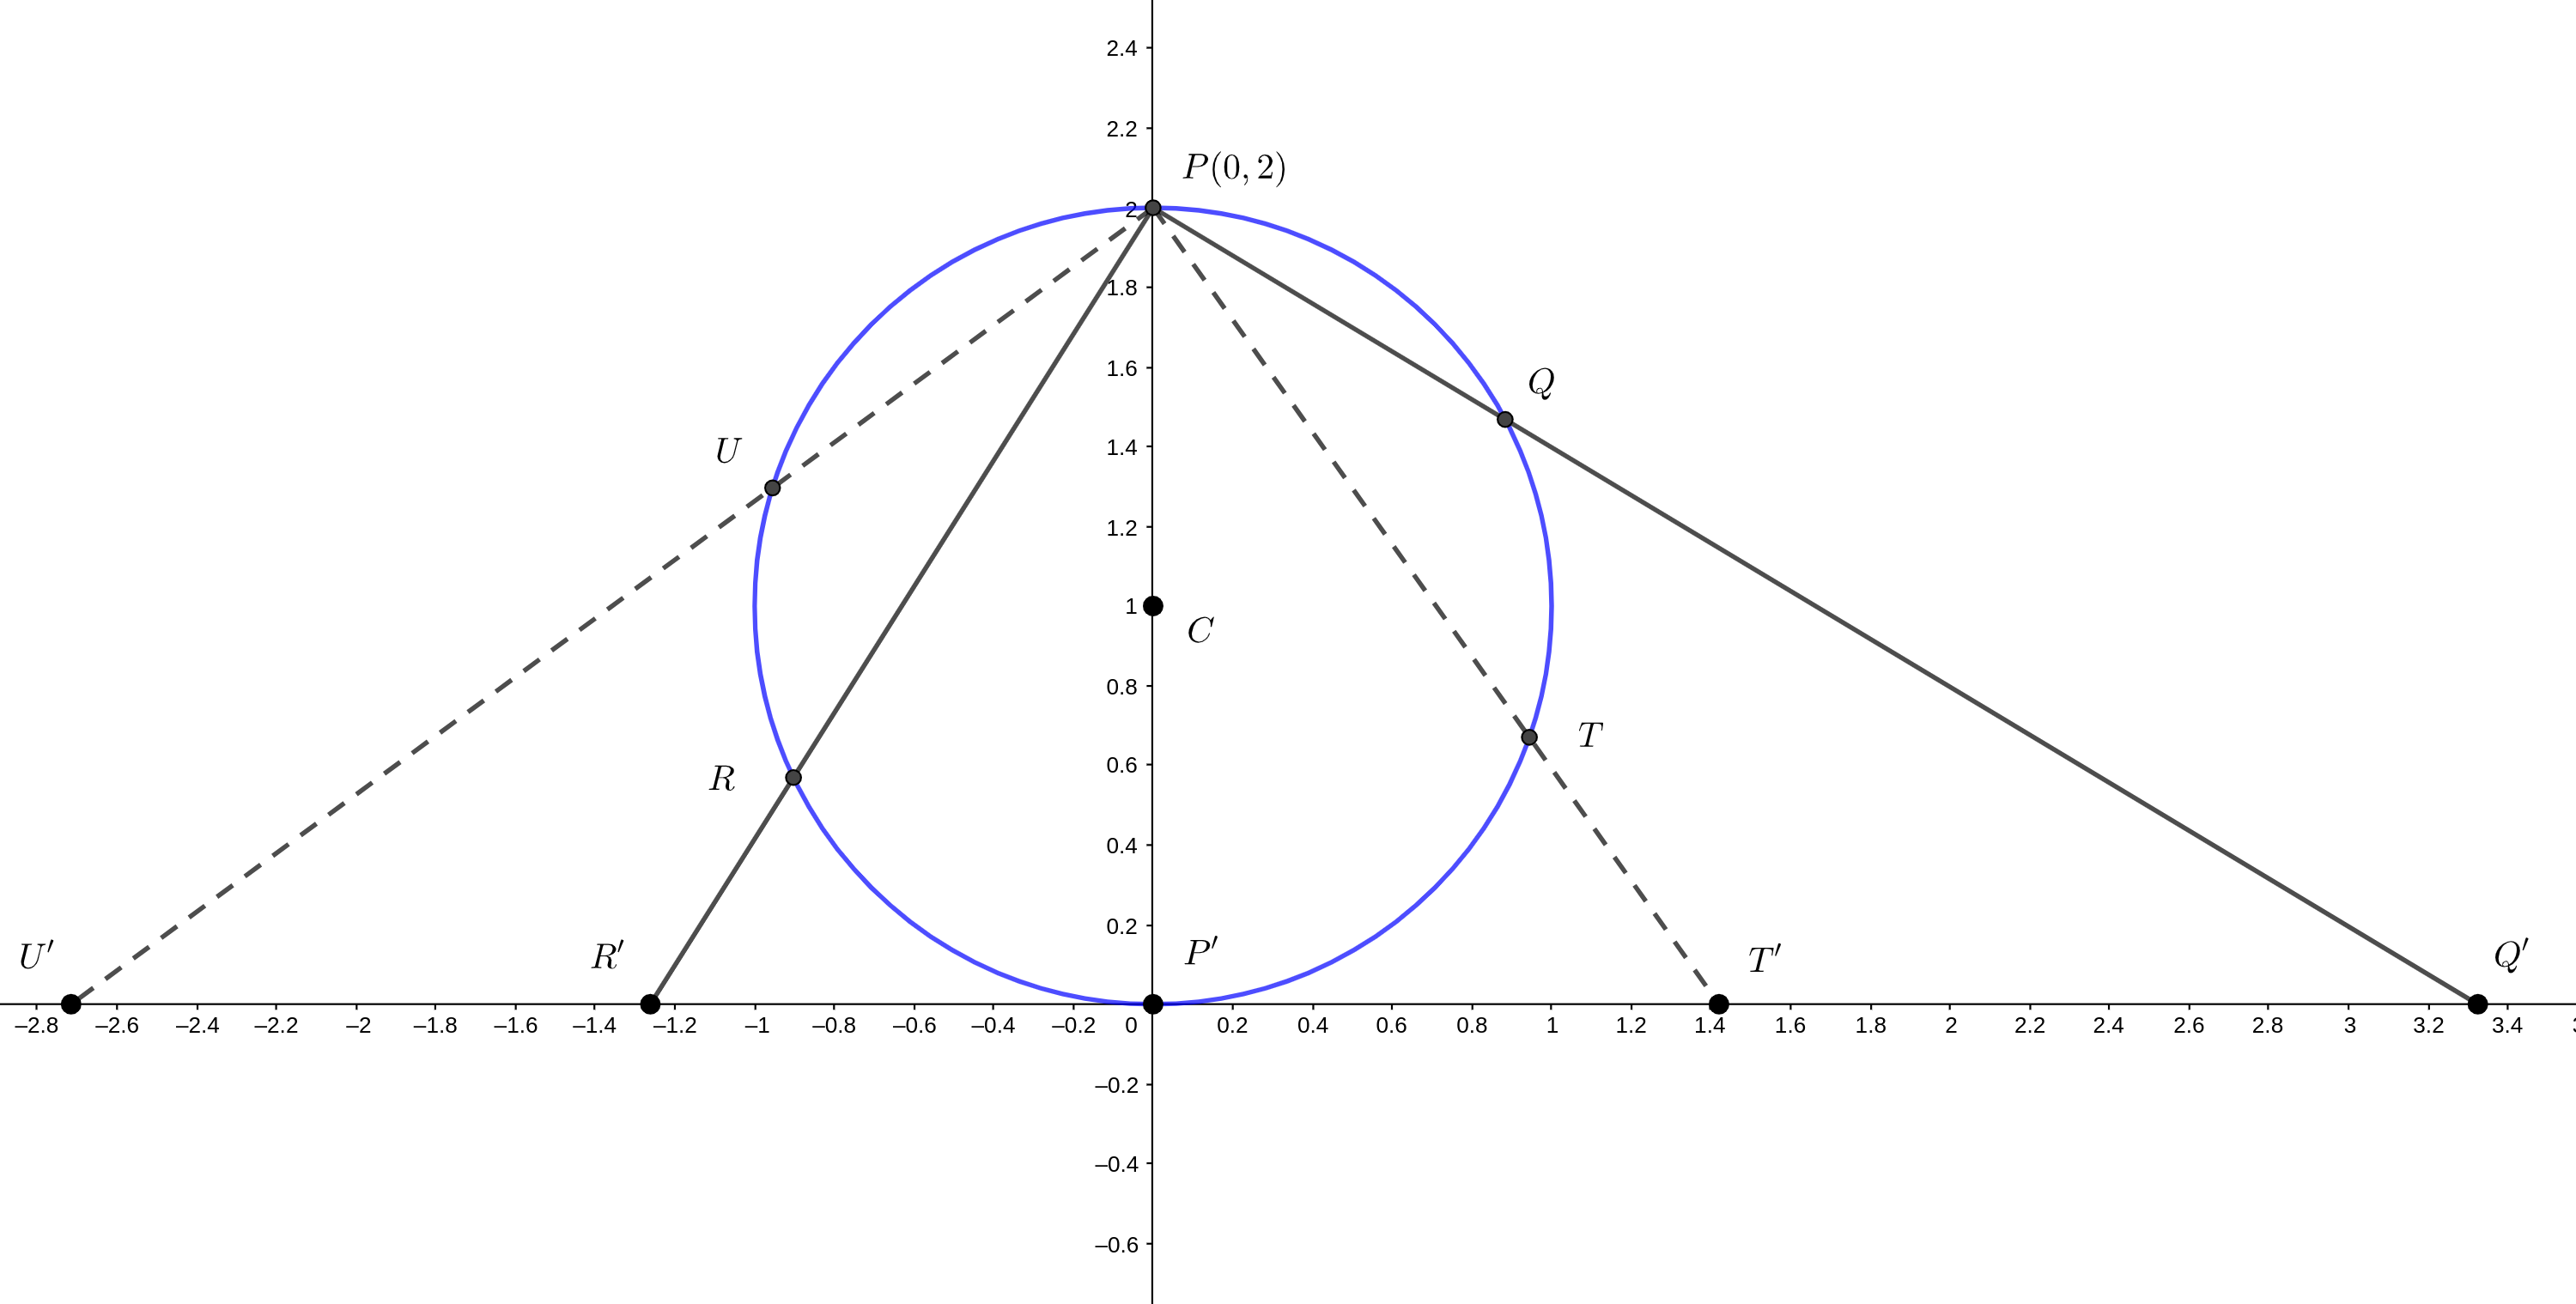
\includegraphics[scale=2]{geogebra-export.png}
    \end{figure}

    This way, we obtain a one-to-one correspondence between the elements of $S$ and the set \(\mathbb{R}\). Hence \(|S| = |\mathbb{R}|\), so $S$ is another uncountable set.

   \subsection{Countable sets}

   \begin{itemize}
       \item \(\mathbb{N} \times \mathbb{N}\) is countable. 
       \begin{proof}
           Define the function \(f: \mathbb{N} \times \mathbb{N} \rightarrow \mathbb{N}\) by \(f(a,b) = 2^a 3^b.\) The result will follow if we can show that $f$ is one-to-one. For \((m,n),(u,v) \in \mathbb{N} \times \mathbb{N}\), \(f(m,n) = f(u,v) \Rightarrow 2^m 3^n = 2^u 3^v \Rightarrow m = u, n = v\). Consequently, $f$ is one-to-one and \(\mathbb{N} \times \mathbb{N}\) is countable. 
       \end{proof}

       \item \(\mathbb{Z} \times \mathbb{Z}\) is countable.
       \begin{proof}
           We know \(\exists g: \mathbb{Z} \rightarrow \mathbb{N}\) bijective. Hence \[g \times g: \mathbb{Z} \times \mathbb{Z} \rightarrow \mathbb{N} \times \mathbb{N}\] is a bijection. But we have \(f: \mathbb{N} \times \mathbb{N} \rightarrow \mathbb{N}\) bijective. Hence \[g \circ (f \times f) : \mathbb{Z} \times \mathbb{Z} \rightarrow \mathbb{N}\] is a bijection.
       \end{proof}

       \item \(\mathbb{Q}\) is countable.
        \begin{proof}
            For \(q \in \mathbb{Q}\), we have \(q = \dfrac{n}{d}\) (reduced) \(\Rightarrow (n,d) \in \mathbb{Z}^2.\)
        \end{proof}
   \end{itemize}

   \emph{Remark:} \(\mathbb{Q}\) is dense in \(\mathbb{R}\). \[x,y \in \mathbb{R} \Rightarrow \exists q \in \mathbb{Q}, x \leq q \leq y.\] \(\mathbb{Q} \times \mathbb{Q}\) is dense in \(\mathbb{R} \times \mathbb{R}\), and \(\mathbb{R} \times \mathbb{R} \setminus \mathbb{Q} \times \mathbb{Q}\) is uncountable.  


   \subsection{Powerset}

   If $A$ is a set, then \(|A| < |\mathcal{P}(A)|.\)

   \begin{proof}
       True if \(A = \emptyset\). If \(A \neq \emptyset\), define \[f:A \rightarrow \mathcal{P}(A).\] $f$ is an injection so \(|A| \leq |\mathcal{P}(A)|.\) Now suppose \(g:A \rightarrow \mathcal{P}(A)\) is a surjection. Define \[B = \{a \in A \mid a \notin g(a)\}.\] Then \(B \subseteq A\), so \(B \in \mathcal{P}(A)\), so \(\exists a \in A\) such that \(g(a) = B\) (g surjective). 
       \begin{itemize}
           \item if \(a \in B\), then \(a \notin g(a)\) so \(a \notin B\).
           \item if \(a \notin B\), then \(a \notin g(a)\) so \(a \in B\). (Contradiction)
       \end{itemize}
   \end{proof}

   \emph{Corollary:} \(|\mathbb{N}| < |\mathcal{P}(\mathbb{N})| < |\mathcal{P}(\mathcal{P}(\mathbb{N}))| < \dots\)
\end{document}